We first analyzed the results in terms of accuracy: how often the models correctly predicted whether a turn transition occurred; in other words, how often the model predicts the correct value of $y_{i+1}$.
%
Table \ref{table:result} shows the results of training a random forest of 200 trees for each model using 10 folds cross validation. We see that using the summary features provides better accuracy than baseline 1, which use only the current dialog act ($65.54\%$ vs $62.79\%$). In addition, using the full model yields an improvement of over $1.08\%$ in the accuracy. In addition, baseline 1 has high precision, it has very low recall. Using only the summary model improves recall and decreases precision by less, leading to a higher F1 score and overall better performance. Using the full model improves precision, which means that dialog acts that were considered to lead to turn transitions are classified correctly. If we use the full model, we lose precision (over baseline 2 model), but gain recall,
leading to the highest F1 score and the best performance.
%
\begin{table}[ht!]
\begin{center}
\begin{tabular}{lrrrrr}
\toprule
{} &  Accuracy &        F1 &  Precision &    Recall &   AUC \\
\midrule
baseline 1 &  0.627938 &  0.578149 &   0.749824 &  0.470491 &  0.659992 \\
baseline 2 &  0.748900 &  0.748792 &   0.818479 &  0.690012 &  0.811185 \\
summary    &  0.655471 &  0.693203 &   0.672255 &  0.713612 &  0.694657 \\
full       &  0.757515 &  0.775993 &   0.775099 &  0.778319 &  0.837863 \\
\bottomrule
\end{tabular}
\end{center}
\caption{Precision, recall and F1 results }
\label{table:result}
\end{table}


The effect can also be seen in figure \ref{auc}, which shows the ROC curves and the AUC for each
model. We notice that the AUC of the summary model is better than baseline 1 model ($0.69$ vs $0.66$), and when adding the summary features to the local features (the full model), we see the AUC improves ($0.84$ vs $0.81$). This suggests that while the discrimination facility of the summary features is lacking (AUC $<0.7$), adding them to a classifier that uses local features (full model) yields better results than the baseline.
%
 \begin{figure}[ht!]
 \centering
 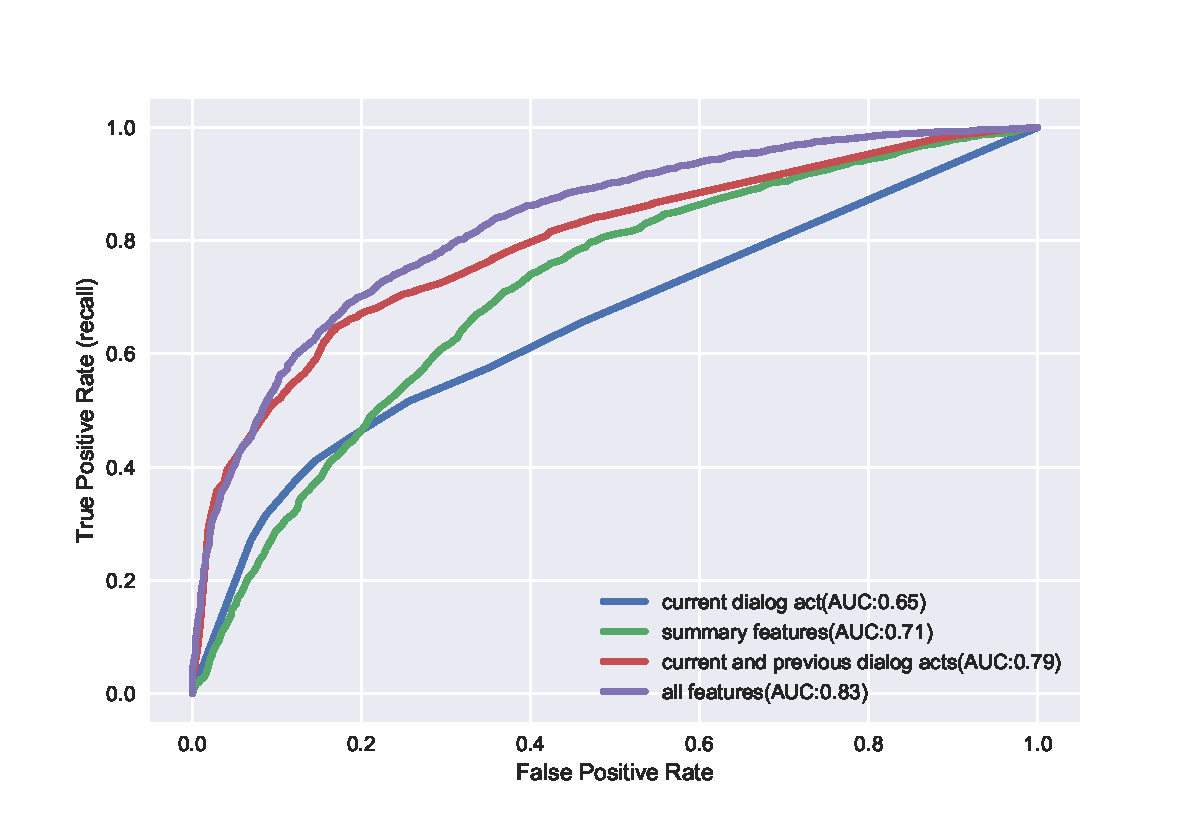
\includegraphics[width=\textwidth]{../scikitlearn/figures/roc.pdf}\vspace{-1.5em}
 \caption{ROC curves and AUC of the different models \label{overflow}}
\label{auc}
 \end{figure}


To measure the affect of time on the conversational image,
we measured the AUC for the four models, using a varying windows sizes from the start of
the conversation. Table \ref{table:starttime} shows the AUC values for different
grouping start time (including a group that contain all the dialog act - starting at time 0).
We can observe that it takes around 30 seconds to reach the maximum AUC when using the baseline model,
while it takes 15 seconds when using all the features. This suggest that as more information
is available to the speaker, it can form an effective turn allocation policy earlier in the conversation.

%
\begin{table}[ht!]
\begin{center}
\begin{tabular}{lrrrrrrr}
\toprule
{} & 0 & 15 & 30 & 45 & 60 & 120 & 180  \\
\midrule
baseline 1 & 0.659992 & 0.661070 & 0.661265 & 0.660901  & 0.660261 & 0.659855 & 0.660598  \\
baseline 2 & 0.811185 & 0.812167 & 0.812493 & 0.812012  & 0.811513 & 0.809206 & 0.806845  \\
summary    & 0.694657 & 0.695172 & 0.694351 & 0.694907  & 0.695737 & 0.691010 & 0.692128  \\
all        & 0.837863 & 0.838777 & 0.838533 & 0.838016  & 0.836148 & 0.831940 & 0.828085  \\

\bottomrule
\end{tabular}
\end{center}
\caption{ AUC Score in relation to the start of the dialog }
\label{table:starttime}
\end{table}

 

